\section{Preliminary}\label{sec:preliminary}

\subsection{Training Process of CNN}
Training of neural network is usually done with stochastic gradient descent. The training process consists of two alternate phases: forward(F) and back-propagation(BP). The forward phase randomly select a batch of training inputs and calculates their inference result with the current model. The backward phase first calculates the error between the inference result and the supervise data of corresponding inputs. Then the error is back-propagated through the network to calculate the gradient of the error to the weights.  

Training of CNN consists of two phases: feed forward (FF) and back propagation. Back propagation phase also consists two steps: calculating neuron gradients (NG) and weight gradients (WG). In this section, we introduce the computation of these three phases for training CNN.\Cref{tab:Notations} summarizes the symbols we use to explain CNN.

\begin{table}[htbp]
    \centering
    \caption{Notations to Explain CNN}
	\begin{tabular}{|l|p{5cm}|}
      \hline
      symbol & description \bigstrut\\
      \hline
      $d ^l$ & The output feature maps of $l^{th}$ layer \bigstrut\\
      \hline
      $\delta ^{l}$ & The error matrix of $l^{th}$ layer \bigstrut\\
      \hline
      $W ^{l}$,$\Delta W^{l}$ & The weights of of $l^{th}$ layer and its gradient. \bigstrut\\
      \hline
      $b ^ l$,$\Delta b ^ l$ & The bias of $l^{th}$ layer and its gradient \bigstrut\\
      \hline
      $ R^l$, $C^l $ & The row and column size of $d ^l$ \bigstrut\\
      \hline
      $ M^l$, $N^l $ & The input and output channel number of $l^{th}$ layer \bigstrut\\
      \hline
      $ K^l $ & The shape of a conv kernel is $K \times K$ \bigstrut\\
      \hline
    \end{tabular}%
    
    \label{tab:Notations}%
  \end{table}%
  
There are three kinds of layers in a typical CNN, \textit{convolutional(CONV) layer, Pooling layer, and fully connected(FC) layer}. Typically convolutional layers process 2-dimensional convolution to extract features. Pooling layers sub-sample the results of CONV layers to reduce the computation time and produce high-level features. The last few layers of a CNN are usually fully connected (FC) layers. FC layers convert the input 3-dimensional feature maps into a long 1-dimensional vector and do Matrix-Vector multiplication to produce output results.
  
\subsubsection{CONV layers}
In feed forward pass, CONV layers calculate 2-D convolution and sum the results of all input channels to produce one output channel. The pseudo code of a convolutional layer can be written as that in Listing \ref{code:conv_forward}.
  
\begin{minipage}{\linewidth}
\begin{lstlisting}[caption=Conv Forward, label=code:conv_forward]  
  for ( row=0; row<`$R^l$`; row++) { 
    for ( col=0; col<`$C^l$`; col++) { 
      for ( to=0; to<`$M^l$`; to++) { 
        `$d^l$`[to][row][col] = `$b^l$`[to];
        for ( ti =0; ti<`$N^l$`; ti++) { 
          for ( i =0; i<`$K^l$`; i++) { 
            for ( j=0; j<`$K^l$`; j++) {
              `$d^l$`[to][row][col] += \
                `$W^l$`[to][ti][i][j] * `$d^{l-1}$`[ti][row+i][col+j];
  } } } } } }

\end{lstlisting}
\end{minipage}

In back propagation pass, $\delta ^{l-1} , \Delta b^l, \Delta W^l$ will be calculated. The pseudo code of a convolutional layer can be written as that in Listing \ref{code:conv_back}. In each loop, the first multiplication accumulation (MAC) operation is in NG step and the second one is in WG step.
    
\begin{minipage}{\linewidth}
\begin{lstlisting}[caption=Conv Back propagation, label=code:conv_back]  
  for ( row=0; row<`$R^{l-1}$`; row++) { 
    for ( col=0; col<`$C^{l-1}$`; col++) { 
      for ( to=0; to<`$M^l$`; to++) { 
        `$\Delta b^{l}$`[to] += `$ \delta ^ l $`[to];
        for ( ti =0; ti<`$N^l$`; ti++) { 
          for ( i =0; i<`$K^l$`; i++) { 
            for ( j=0; j<`$K^l$`; j++) {
              `$\delta ^ {l-1}$`[ti][row][col] += \
                `$W^l$`[to][ti][i][j] * `$\delta ^ {l}$`[to][row-i][col-j] ;
              `$\Delta W^l$`[to][ti][i][j] += \
                `$\delta ^l$`[to][row-i][col-j] * `$d ^ {l-1} $`[ti][row][col];
  } } } } } }

\end{lstlisting}
\end{minipage}

\subsubsection{FC layers} \label{sec:prelim:fc}

All the elements in the input feature or output feature can be considered in a vector. The length of the input vector is $M$, and the output vector length is $N$. The forward process can be described in Listing \ref{code:fc_forward}.

\begin{minipage}{\linewidth}
\begin{lstlisting}[
  caption=FC Forward,
  label=code:fc_forward]
  for ( to=0; to<`$M$`; to++ ) {
    `$d^l$`[to] += `$b^l$`[to];
    for ( ti =0; ti<`$N$`; ti++) {
      `$d^l$`[to] += `$d^{l-1}$`[ti] * `$W$`[to][ti];
} }
\end{lstlisting}
\end{minipage}

As same as CONV layers,  $\delta ^{l-1} , \Delta b^l, \Delta W^l$ will be calculated in back propagation pass. The back propagation of FC layer is shown in Listing \ref{code:fc_backpropagation}.

\begin{minipage}{\linewidth}
\begin{lstlisting}[
  caption=FC Back propagation,
  label=code:fc_backpropagation]
for ( ti =0; ti<N; ti++ ){
  `$\Delta b^l$`[ti] = `$\delta ^ l$`[ti];
  for ( to=0; to<M; to++ ) {
    `$\delta ^ {l-1}$`[ti] += `$W$`[to][ti] * `$\delta ^ l$`[to];     
    `$\Delta W ^ l$`[ti][to] = `$d^{l-1}$`[ti]*`$\delta ^ l$`[to];
} }
\end{lstlisting}
\end{minipage}

\subsubsection{Pooling layers}
In FF phase, pooling layers down samples each channel of the input feature map. There are no weights for Pooling layers to train. A typical down sampling function is the max pooling function, which is to find the maximum value of small windows of the input feature maps. No WG step is needed for pooling layer. For NG step, a pooling layer upsamples the error according to the downsampling function. \Cref{fig:pool} illustrates an example of FF and NG step of a $2\times 2$ max pooling layer.
\begin{figure}[htbp]
    \centering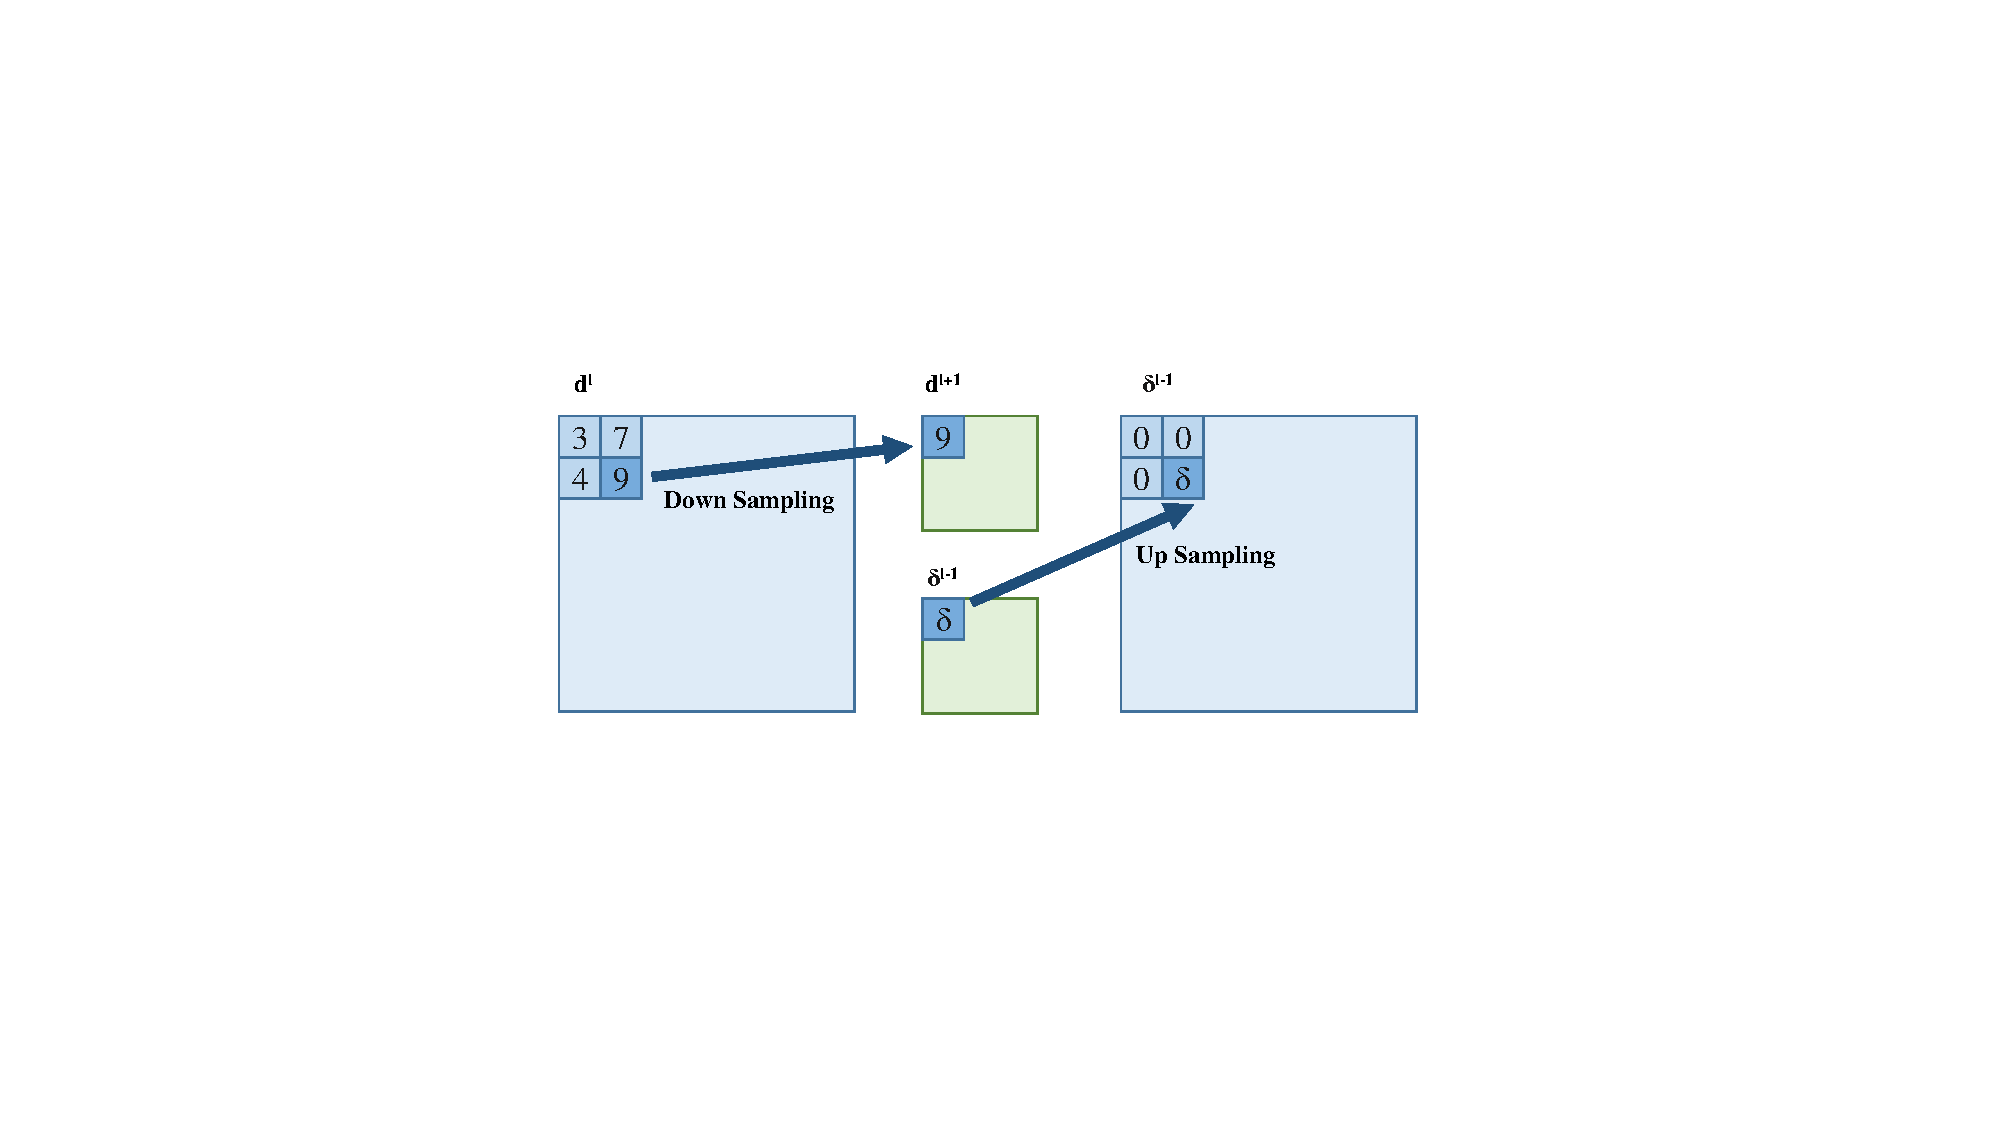
\includegraphics[width=3.2in]{figures/pool.pdf}
    \caption{Example of a $2\times 2$ max pooling layer}\label{fig:pool}
\end{figure}